% $Header: /Users/joseph/Documents/LaTeX/beamer/solutions/generic-talks/generic-ornate-15min-45min.en.tex,v 90e850259b8b 2007/01/28 20:48:30 tantau $

\documentclass[utf8]{beamer}

\usepackage{tikz}
\usetikzlibrary{arrows}
\usetikzlibrary{positioning}
\usetikzlibrary{shapes}
\usetikzlibrary{decorations.pathmorphing}

% This file is a solution template for:

% - Giving a talk on some subject.
% - The talk is between 15min and 45min long.
% - Style is ornate.



% Copyright 2004 by Till Tantau <tantau@users.sourceforge.net>.
%
% In principle, this file can be redistributed and/or modified under
% the terms of the GNU Public License, version 2.
%
% However, this file is supposed to be a template to be modified
% for your own needs. For this reason, if you use this file as a
% template and not specifically distribute it as part of a another
% package/program, I grant the extra permission to freely copy and
% modify this file as you see fit and even to delete this copyright
% notice. 


\mode<presentation>
{
  \usetheme{CambridgeUS}
  \usecolortheme{dolphin}


  \setbeamercovered{transparent}
  % or whatever (possibly just delete it)
}

\usepackage[english]{babel}
\usepackage[utf8]{inputenc}

\usepackage{libertine}
\usepackage[T1,T2A]{fontenc}

\usebackgroundtemplate%
{%
    
\includegraphics[width=\paperwidth,height=\paperheight]{grnet_background.pdf}%
}


\title[e-Voting and Zeus]{e-Voting from the Ground Up and Zeus}

\author[Panos Louridas]{Panos Louridas}
\date[EESTEC Workshop]{March 14, 2013 / EESTEC Govern the Way of Youth 2013}
\institute[GRNET]{Greek Research and Technology Network (GRNET) S.A.}

\subject{Talks}
% This is only inserted into the PDF information catalog. Can be left
% out. 

% If you have a file called "university-logo-filename.xxx", where xxx
% is a graphic format that can be processed by latex or pdflatex,
% resp., then you can add a logo as follows:

% \pgfdeclareimage[height=0.5cm]{university-logo}{university-logo-filename}
% \logo{\pgfuseimage{university-logo}}


% Delete this, if you do not want the table of contents to pop up at
% the beginning of each subsection:
\AtBeginSubsection[]
{
  \begin{frame}<beamer>{Outline}
    \tableofcontents[currentsection,currentsubsection]
  \end{frame}
}


% If you wish to uncover everything in a step-wise fashion, uncomment
% the following command: 

%\beamerdefaultoverlayspecification{<+->}


\begin{document}

\begin{frame}
  \titlepage
\end{frame}

\begin{frame}{Outline}
  \tableofcontents
  % You might wish to add the option [pausesections]
\end{frame}

\section{Paper Ballots}

\subsection{Advantages}

\begin{frame}{Why Paper Ballots?}{A lot going for them.}

  \begin{itemize}
  \item Long experience (how long have we been using them?)
  \item Low tech solution (for those running the election)
  \item No skills required (at most reading and writing, and then
    again not always)
  \item There is an underlying physical asset \pause the ballot itself
  \item People may actually enjoy election day
  \end{itemize}

\end{frame}

\begin{frame}{What If\ldots}{Something Goes Wrong?}

  \begin{itemize}
  \item<1->Can I prove that I have voted?
    \pause Yes
  \item<2->Is my vote anonymous?
    \pause Yes
  \item<3->Have all votes been counted?
    \pause Yes
  \item<4->Has my vote been counted?
    \pause Yes
  \item<5->It is possible to add votes?
    \pause No
  \item<5->It is possible to falsify votes?
    \pause No
  \end{itemize}

\end{frame}

\begin{frame}{Underlying Assumptions}{That We Usually Take for Granted}

  \begin{itemize}
  \item<1->The election authorities are trustworthy and independent
  \item<2->Favourable political climate
  \item<3->Logistics have been solved \pause or we may need to call in
    international monitors etc.
  \end{itemize}

\end{frame}

\subsection{Disadvantages}

\begin{frame}{Why Then Consider e-Voting?}{Issues with Paper Ballots}

  \begin{itemize}
  \item Logistics are cumbersome
  \item Cost
  \item Not everybody is able to go to the ballot box
  \item Counting can take a long time and is boring
  \item The underlying physical asset (the ballot) is vulnerable to
    physical destruction (fire, water, theft,\ldots)
  \end{itemize}

\end{frame}

\section{Requirements for an e-Voting System}

\begin{frame}{Democratic}

  \begin{itemize}
  \item Only eligible voters can vote.
  \item Each eligible voter can cast at most one vote (that counts).
  \end{itemize}

\vfill

Source of e-Voting System Requirements:
\url{http://courses.csail.mit.edu/6.897/spring04/L17.pdf}

\end{frame}


\begin{frame}{Private}

  \begin{itemize}
  \item No one can tell how a voter actually voted (anonymity, at
    least within large enough cohort/precinct of voters).
  \item OK (perhaps even mandatory) to publish who voted (though,
    obviously not actual ballot content).
  \end{itemize}

\end{frame}

\begin{frame}{Uncoercible}

  \begin{itemize}
  \item Voter cannot be coerced or bribed to vote a particular way.
  \item Voter cannot prove how they voted to another party:
    receipt-free. (Note how this requirement assumes the voter may be
    an adversary.)
  \end{itemize}
  
\end{frame}

\begin{frame}{Accurate}

  The final tally is the correct sum of cast votes.
  \begin{itemize}
    \item Cast ballots can't be altered, deleted, substituted.
    \item All cast ballots are counted; other (invalid) ballots can't
      be added.
    \end{itemize}
  
\end{frame}

\begin{frame}{Verifiable}

  \begin{quote}
  I consider it completely unimportant who in the party
  will vote, or how; but what is extraordinarily important is
  this---who will count the votes, and how. 
  \end{quote}
  Joseph Stalin 

  In Russian: Я считаю, что совершенно неважно, кто и как будет в
  партии голосовать; но вот что чрезвычайно важно, это---кто и как
  будет считать голоса. 

  Said in 1923, as quoted in The Memoirs of Stalin's Former Secretary
  (1992) by Boris Bazhanov [Saint Petersburg] (Борис Бажанов.
  Воспоминания бывшего секретаря Сталина). 

  Variant (loose) translation: The people who cast the votes decide
  nothing. The people who count the votes decide everything.

\end{frame}

\begin{frame}{Verifiable}

\begin{itemize}
\item Individual verifiability: each voter may verify their vote.
\item Representative verifiability: each voter may delegate to a party
  or other representative the task of verifying the vote (without
  revealing the vote in the clear, of course).
\item Universal verifiability: anyone can verify total.
\end{itemize}

\end{frame}

\begin{frame}{Robust}

\begin{itemize}
\item A small group can't disrupt election (DOS attacks, complaint
  procedures, etc\ldots)
\end{itemize}

\end{frame}

\begin{frame}{Fairness}

\begin{itemize}
  \item No partial results are known before the election is closed.
  \end{itemize}
  
\end{frame}

\begin{frame}{Ease of Use}

\begin{itemize}
  \item Good user interface
  \item Accessibility and usability guidelines
  \item Accessibility from a wide variety of input devices
\end{itemize}

\end{frame}

\begin{frame}{Efficiency}

  \begin{itemize}
  \item Efficient ballot casting
  \item Efficient ballot counting
  \end{itemize}
  
\end{frame}

\section{The Helios Voting System and Process}

\begin{frame}{Helios v. 1 Workflow}

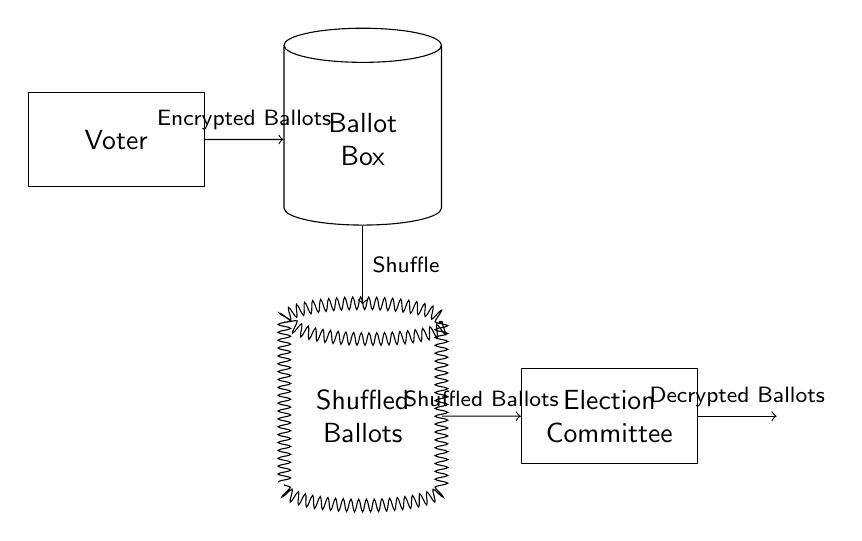
\begin{tikzpicture}[font=\sffamily]
  \tikzset{ballotbox/.style={cylinder, shape border rotate=90,
      text width=1.5cm,
      minimum height=2.5cm,
      minimum width=2cm,
      aspect=0.25, 
      align=center,
      draw}}
  \tikzset{shuffled/.style={cylinder, shape border rotate=90,
      text width=1.5cm,
      minimum height=2.5cm,
      minimum width=2cm,
      aspect=0.25, 
      align=center,
      decorate, 
      decoration={snake, amplitude=0.08cm, segment length=0.1cm},
      draw}}
  \tikzset{person/.style={rectangle, text width=2cm, text centered, 
      minimum height=1.2cm, draw}}
  \tikzset{to/.style={->,font=\sffamily\footnotesize}},
  \node[person] (voter) {Voter};
  \node[ballotbox] (ballotbox) [right=of voter]{Ballot Box};
  \node[shuffled]  (shuffled) [below=of ballotbox] {Shuffled Ballots};
  \node[person] (committee) [right=of shuffled] {Election Committee};
  \node (results) [right=of committee] {};
  \draw[to] (voter) -- node[midway,above]{Encrypted Ballots} (ballotbox);
  \draw[to] (ballotbox) -- node[midway,right]{Shuffle} (shuffled);
  \draw[to] (shuffled) -- node[midway,above]{Shuffled Ballots} (committee);
  \draw[to] (committee) -- node[midway,above]{Decrypted Ballots} (results);
\end{tikzpicture}

\end{frame}

\begin{frame}{Basic Ideas}

\begin{itemize}
\item Ballots are encrypted on the browser before being sent to the
  server.
\item Ballots are stored in the server in encrypted form.
\item The decryption keys are kept by the Election Committee.
\item Encrypted ballots are randomly mixed in order to break the
  association between ballots and voters.
\item The encrypted mixed ballots are decrypted by the Election
  Commitee.
\item The process can be verified mathematically.
\end{itemize}

\end{frame}

\begin{frame}{Basic Assumptions}

\begin{itemize}
\item You do not need to trust the administrators of Helios.
\item You do not need to trust each member of the Election Committee.
\item You need to trust that at least one member of the Election
  Committee is honest.
\item Coercion is avoided by allowing multiple ballots per user (only
  the last one counts).
\end{itemize}

\end{frame}

\section{How Does it Work?}

\begin{frame}{Public Key Cryptography}

 \begin{columns}[t]
   \column{.48\textwidth}
   Alice
   \begin{enumerate}
   \item<1-> Alice chooses a number, say 3, and keeps it secret. We
     label her number $A$.
   \item<2-> Alice puts 3 into the one-way function $y^x\pmod p =
     7^x\pmod 11$ and works out the result of $7^3\pmod{11} = 2$.
   \item<3-> Alice calls the result of this calculation $\alpha$ and
     sends it to Bob.
   \item<4-> Alice takes Bob's result and works out the result of
     $\beta^A\pmod{11} = 9$.
   \end{enumerate}

  \column{.48\textwidth}
  Bob
  \begin{enumerate}
  \item<1-> Bob chooses a number, say 6, and keeps its secret. We
    label his number $B$.
  \item<2-> Bob puts 6 into the one-way function and works out the
    result of $7^6\pmod{11} = 4$.
  \item<3-> Bob calls the result of this calculation $\beta$ and
    sends it to Alice.
  \item<4-> Bob takes Alice's resut, and works out the result of
    $\alpha^B\pmod{11} = 9$.
  \end{enumerate}  
\end{columns}

\end{frame}

\begin{frame}{ElGamal}{Key Generation}

  \begin{enumerate}
    \item Choose a prime, $p$, and two random numbers $g$ and $x$ such
      that both $g$ and $x$ are less than $p$.
    \item Calculate $y = g^x\pmod{p}$
    \item The public key is $y$, $g$, and $p$. Both $g$ and $p$ can be
      shared among a group of uses. 
    \item The private key is $x$.

  \end{enumerate}

Source of ElGamal key generation, encryption, decryption: Bruce
Schneier, Applied Cryptography, 2nd ed., 1996.

\end{frame}

\begin{frame}{ElGamal}{Encryption}

  \begin{enumerate}
    \item To encrypt message $M$, first choose a random $k$, such that
      $k$ is relatively prime to $p - 1$.
    \item Compute $a = g^k\pmod{p}$ and $b = y^kM\pmod{p}$. The pair
      $(a, b)$ is the cyphertext.
    \end{enumerate}
  \end{frame}

\begin{frame}{ElGamal}{Decryption}

  \begin{itemize}
  \item Compute $M = b / a^x\pmod{p}$.
  \end{itemize}
  
  This holds since:
  \[ a^x = g^{xk}\pmod{p} \]
  and 
  \[ b/a^x = y^kM/a^x = g^{xk}M/g^xk = M\pmod{p} \]

\end{frame}

\begin{frame}{ElGamal}{Re-encryption}

  \begin{enumerate}
  \item Take a ciphertext $c = (a, b)$.
  \item Select $s$ such that it is less than $p$.
  \item Compute $c' = (g^sa, y^sb)$.
  \item If we decrupt $c'$ we get:
    \[y^sb / (g^sa)^x = g^{xs}y^kM / g^{sx}a^x = y^kM / a^x = g^{xk}M/g^xk =
    M\pmod{p} \]
  \end{enumerate}
    
\end{frame}

\begin{frame}[c]{Zero Knowledge Proof of Knowledge}

  \includegraphics<1>[width=\textheight]{Zkip_alibaba1.png}
  \includegraphics<2>[width=\textheight]{Zkip_alibaba2.png}
  \includegraphics<3>[width=\textheight]{Zkip_alibaba3.png}

Source: \url{http://en.wikipedia.org/wiki/Zero-knowledge_proof}

\end{frame}

\section{From Helios to Zeus}

\begin{frame}{Helios Combines Ballot Counting with Election Results}

  \begin{itemize}
  \item Helios combines ballot counting with producing the election
    results.
  \item After the first version uses homomorphic encryption, so no
    mixnets are used.
  \end{itemize}

\end{frame}


\begin{frame}{Zeus Separates Ballot Counting from Election Results}
  
  \begin{theorem}
    We can have secure elections even when ballot counting and election
    results are separated.
  \end{theorem}

\begin{proof}
  \begin{enumerate}
  \item<1-> Ballot counting can be verified, using the same mathematics
    as in Helios.
  \item<2-> Production of the final results can be verified since it is
    an open process. Hence the whole elections can be verified.\qedhere
  \end{enumerate}
\end{proof}

\end{frame}

\section{Zeus Elections to Date}

% \section*{Summary}

% \begin{frame}{Summary}

%   % Keep the summary *very short*.
%   \begin{itemize}
%   \item
%     The \alert{first main message} of your talk in one or two lines.
%   \item
%     The \alert{second main message} of your talk in one or two lines.
%   \item
%     Perhaps a \alert{third message}, but not more than that.
%   \end{itemize}
  
%   % The following outlook is optional.
%   \vskip0pt plus.5fill
%   \begin{itemize}
%   \item
%     Outlook
%     \begin{itemize}
%     \item
%       Something you haven't solved.
%     \item
%       Something else you haven't solved.
%     \end{itemize}
%   \end{itemize}
% \end{frame}

\end{document}
